\documentclass{article}
\usepackage[margin=3cm]{geometry}
\usepackage{amssymb}

% Figures
\usepackage{graphicx}
\usepackage{color}

% Page formatting
\newsavebox{\notetitle}
\newsavebox{\noteauthor}
\newsavebox{\notenumber}
\newsavebox{\notedate}

\renewcommand{\title}[1]{\sbox{\notetitle}{\begin{minipage}{1.0\textwidth} \begin{center} \Large{\textbf{#1}} \end{center}\end{minipage} }}
%\renewcommand{\author}[1]{\renewcommand{\and}{\quad}\sbox{\noteauthor}{\large{#1}}}
\renewcommand{\author}[1]{\sbox{\noteauthor}{\begin{minipage}{1.0\textwidth} \begin{center} \large{#1} \end{center}\end{minipage}}}
\renewcommand{\date}[1]{\sbox{\notedate}{\large{#1}}}
\newcommand{\nb}[1]{\sbox{\notenumber}{\Large{\textbf{#1}}}}

\newcommand{\makemadtitle}{
  \hrule
  \vspace{.5em}
  \noindent
  \begin{center}
  \textbf{
  {\centering
\includegraphics[height=3cm,bb=0 0 371 145]{../logoCHISTERA2014.png}}\\
  %{\centering
\includegraphics[height=3cm]{../logoCHISTERA2014.eps}}\\
   {\centering\Large COACHES project, CHIST-ERA 2014 program}
  }
  \end{center}
  \vspace{.5em}
 
  \hrule
  \vspace{3em}
  \begin{center}
    %\begin{large}\textbf{ Note~\usebox{\notenumber}.}\end{large}\\[.5em]
    \begin{Large}\textbf{\usebox{\notetitle}}\end{Large}\\[2em]
    \begin{large}\usebox{\noteauthor}\\ [2em]
    \usebox{\notedate}\end{large}
  \end{center}
  \vspace{3em}
}

% Various macros and environments
\newtheorem{prop}{Proposition}
\newtheorem{proposition}[prop]{Proposition}
\newtheorem{defn}{Definition}
\newtheorem{definition}[defn]{Definition}
\newtheorem{cor}{Corollary}
\newtheorem{corollary}[cor]{Corollary}
\newtheorem{exmp}{Example}
\newtheorem{example}[exmp]{Example}
\newtheorem{lem}{Lemma}
\newtheorem{lemma}[lem]{Lemma}
\newtheorem{fact}{Fact}
\newtheorem{thm}{Theorem}
\newtheorem{theorem}[thm]{Theorem}
\newtheorem{prob}{Problem}
\newtheorem{problem}[prob]{Problem}
\newtheorem{rem}{Remark}
\newtheorem{remark}[rem]{Remark}
\newtheorem{conj}{Conjecture}
\newtheorem{conjecture}[conj]{Conjecture}
\newenvironment{pf}{{\bf Proof }}{\hfill$\Box$\par}
\newenvironment{proof}{{\bf Proof }}{\hfill$\Box$\par}
\newcommand{\spaceafterproof}{\vspace{1em}}

% NOTE ITSELF BELOW %%%%%%%%%%%%%%%%%%%%%%%%%%%%%%%%%%%%%%%%%%%%%

\title{D5.1\\ Definition of internal architecture and interface between software modules}

\author{Domenico D. Bloisi, Fabio Maria Carlucci, Luca Iocchi, Daniele Nardi\\
Dept. of Computer, Control and Management Engineering\\
Sapienza University of Rome, Italy}


%\nb{of the kickoff meeting, $27^{th},28^{th}$ October }

\date{December 30, 2014}

\begin{document}


\includegraphics[height=3cm]{../logoSapienza.png}

\makemadtitle

\begin{abstract}
This document describes the software architecture of the entire project, showing the main software components, their connections and the interfaces between them.
\end{abstract}

\vspace*{4.0cm}

\fbox{
\begin{minipage}{1.0\textwidth}
\begin{center}
 $\copyright$, THE COACHES CONSORTIUM \\
The copyright in this document is the property of the COACHES Consortium. This document is supplied by the COACHES consortium on the express terms that it is to be treated as confidential. This document is not external distribution without the project manager's permission. 
\end{center}
\end{minipage}
}
\newpage

\begin{figure}
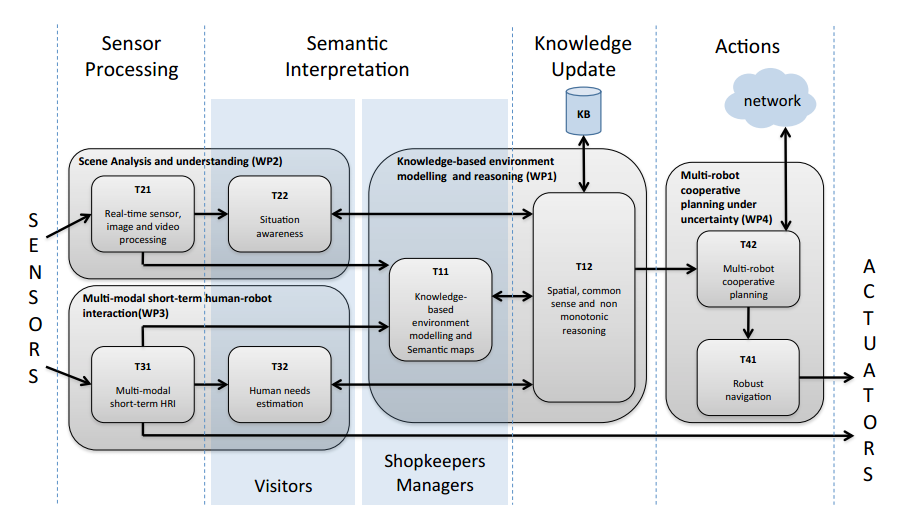
\includegraphics[width=0.95\textwidth]{COACHES_swarch.png}
\caption{COACHES software architecture}
\label{fig:swarch}
\end{figure}

\section{Introduction}

In this document we describe the software architecture of the COACHES project.

We describe our choice regarding the middleware chosen to implement the entire system.  Moreover,  we  precisely  define  the  interface 
between  each  pair  of  modules  connected by  a  flow  of  information  as  depicted  in 
Figure \ref{fig:swarch}. 
Subsequent implementation of the software components during the project will follow  these  specifications,  thus  simplifying  their  integration  in  the demonstrators. 

We will use an open architecture (hard/soft) and standard technologies available (such 
as ROS for integrating robotic modules and DDS for communication) so that it will be 
easy to extend and/or adapt the capabilities of the system during the whole length of 
the  project  (especially  to  integrate  and  test  various  algorithms  and/or  sensors).  Such 
an open architecture will also simplify and optimize integration efficiency as well as re-use of assets in other projects or products. 

In the following of this document, we will first describe the choice of the middleware, then the main software components and the  set-up of a 2D simulation environment for testing the developments, finally we describe the version management system that will be used to manage the development.

\section{Middleware}

For the development of the software robotics components, we use the Robot Operating System (ROS) (www.ros.org), which is the standard middleware for robotics applications.
In particular, we will use the last stable version ROS Indigo and the last LTS (Long Term Support) version of the Linux/Ubuntu Operating System.

ROS provides the middleware to share information among the many modules implementing various functionalities on each robot. Moreover, an interface (ROS-through-TCP) will be realized in order to share information among the robots and between each robot and other components of the system.

\section{Main software components}

In this section we describe the main robotic software components that will be development for the control, the reasoning and the interaction functionalities of the robot.

\subsection{Robotic software components}

The main robotic software components that will be realized within the COACHES project are related to the following project tasks.
\begin{itemize}
\item T1.1 KB modeling
\item T1.2 KB reasoning
\item T2.1 Image Processing
\item T2.2 Situation Awareness
\item T3.1 Multimodal HRI
\item T3.2 Human needs estimation
\item T4.1 Robust navigation
\item T4.2 Multi-robot planning
\end{itemize}

Sapienza University is responsible for tasks T3.1 and T4.1.


\section{2D Simulation Environment}


\section{Version management system}

In order to manage the development of the software by all the partners of the project, we have supported the team from University of Caen in the set up of a GIT repository for the software.
The repository is accessible only by the project partners and it is organized as follows.

The 'coaches/software' folder contains source code, libraries and binary code 
divided in the following sub-folders:

\begin{itemize}
\item \emph{src}:       contains (non-ROS) source code maintained in the coaches repository
\item \emph{ros}:       contains ros modules
\item \emph{external}:  contains external software not maintained in the coaches repository
\item \emph{bin}:       contains executable files
\item \emph{include}:   contains include files 
\item \emph{lib}:       contains libraries
\end{itemize}

Automated scripts for initializing, setting-up, updating, building and testing the software environment have been developed and described in the repository. These scripts will facilitate updates and testing and thus in  general the integration of functionalities developed by the different developers.

The \emph{ros} folder contains a Catkin workspace (which is the standard building environment in ROS) and the following ROS packages, including the robotic software components described above.

\begin{itemize}
\item \emph{hello\_coaches\_developers}: a test package to check correct installation and set-up of the environment;
\item \emph{t11\_kb\_modeling}: software developed for Task T1.1;
\item \emph{t12\_kb\_reasoning}: software developed for Task T1.2;
\item \emph{t21\_image\_processing}: software developed for Task T2.1;
\item \emph{t22\_situation\_awareness}: software developed for Task T2.2;
\item \emph{t31\_multimodal\_hri}: software developed for Task T3.1;
\item \emph{t32\_human\_needs\_estimation}: software developed for Task T3.2;
\item \emph{t41\_robust\_navigation}: software developed for Task T4.1;
\item \emph{t42\_multi\_robot\_planning}: software developed for Task T4.2;
\end{itemize}


Moreover, additional packages developed outside the COACHES project are present in the \emph{external} directory and linked in the ROS Catkin workspace.
Some examples of these external packages are:
\begin{itemize}
\item \emph{gradient\_based\_navigation}: a package for safe navigation and obstacle avoidance in dynamic environments;
\item \emph{PetriNetPlans}: library and ROS bridge for plan execution;
\item \emph{stage\_environments}: a package for 2D simulation.
\end{itemize}



\end{document}
